\part{Advanced features}
\section{Targets}
\label{sec:Targets} Target option -t provides an easy way to identify, by means of a regular
expression, a particular log trace in your logs. By default, it will tail as
normal and if your regex is matched, then that line will be emphasized in a red
background.\\
Example:\\
\emphlogtrace{this is a log trace matched by target option}

You can specify multiple comma separated targets. Each target is just an string being 
itself a simple string or just a regular expression. It must be enclosed within simple or 
double quotes.
\begin{cmd}
 ./log4tail -t [--target] 'regex1,regex2,regex3,...,regexN' pathToLogs
\end{cmd}

\subsection{Every log with its own target scheme}
If you want every log with its own targets, then you must provide them in a config file. 
In order to do that, just edit a text file and specify the next key, value optional parameters:
\begin{verbatim}
targets fullpathToLog0 = regex0, regex1,.., regexN | colorregex0,.., coloregexN
targets fullpathToLog1 = regex0, regex1,.., regexN | colorregex0,.., coloregexN
\end{verbatim}
An example of that could be:
\begin{verbatim}
targets /var/log/messages = iptables$, ^2009-08-07 user | blue, red
targets /var/log/mail.log = incoming \d+, \d{1,3} something | on_cyan
\end{verbatim}
If an specific regex does not have a corresponding color, then it will be emphasized using
the default color setup, which is the log trace on a red background.



\section{Throttling}
In release v05, the throttling option is provided. Many applications when
started usually tend to upload configuration parameters and log them very fast,
which makes nearly impossible to identify anything (unless you open the log and
check). In that case, or in other ones where an application logs very fast, you
can provide the \emph{throttle} option specifying the number of seconds you want
to output in the screen the logging information one line at a time. The number 
of seconds can be a floating point number.
\begin{cmd}
 ./log4tail --throttle 0.5 pathToLogs
\end{cmd}
That would tail the logs showing the information every half a second one line at 
a time.


\section{Notifications}
\logftailer{} uses \emph{Notifications} to identify what kind of action needs to
trigger when it matches a certain line with an specific log4j level. The actions
provided as of version v05 are:
\begin{itemize}
 \item Print (see \autoref{sec:PrintAction})
 \item Filter (see \autoref{sec:filter})
 \item CornerMark (see \autoref{sec:cornermark})
 \item Mail (see \autoref{sec:mailnotification})
 \item Inactivity (see \autoref{sec:inactivitysection})
 \item Executor (see \autoref{sec:executor})
 \item Poster (see \autoref{sec:poster})
\end{itemize}

\subsection{Print Notification}
\label{sec:PrintAction}PrintAction does what the famous \emph{tail} command does, just printing in the
screen (terminal) but with colors. When an application logs information very
fast, colors provide and easy way to quickly identify a certain pattern or
problem. Every color identify an specific level according to the log4j java
framework.

\subsubsection{Available colors}
\logftailer{} provides the following foreground colors:

\begin{center}
\begin{tabular}{|l || c|}
\hline
 black (default for debug) & {\color{black} \textbf{This is a test logtrace}} \\ 
\hline
 red (default for fatal and critical) & {\color{red} \textbf{This is a test logtrace}} \\ 
\hline
 green (default for info) & {\color{green} \textbf{This is a test logtrace}} \\ 
\hline
yellow (default for warning) & {\color{yellow} \textbf{This is a test logtrace}} \\ 
\hline
 blue & {\color{blue} \textbf{This is a test logtrace}} \\ 
\hline 
magenta (default for error) & {\color{magenta} \textbf{This is a test logtrace}} \\ 
\hline
 cyan & {\color{cyan} \textbf{This is a test logtrace}} \\ 
\hline 
white & \colorbox{black}{\color{white}\textbf{This is a test logtrace}} \\
\hline
\end{tabular}
\end{center}

and the additional background colors:
\begin{center}
\begin{tabular}{|l | c |}
  \hline
 on\_black & \colorbox{black}{\color{green}this is a test logtrace} \\
 \hline
 on\_red & \colorbox{red}{this is a test logtrace} \\
 \hline
on\_green & \colorbox{green}{this is a test logtrace} \\
 \hline
on\_yellow & \colorbox{yellow}{this is a test logtrace} \\
 \hline
 on\_blue & \colorbox{blue}{this is a test logtrace} \\
 \hline
 on\_magenta & \colorbox{magenta}{this is a test logtrace} \\
 \hline 
on\_cyan & \colorbox{cyan}{this is a test logtrace} \\
 \hline 
on\_white & \colorbox{white}{this is a test logtrace} \\
\hline
\end{tabular}
\end{center}

%\begin{itemize}
 %\item on\_black \hspace{20pt}\colorbox{black}{\color{green}this is a test logtrace}
 %\item on\_red \hspace{29pt}\colorbox{red}{this is a test logtrace}
 %\item on\_green \hspace{20pt}\colorbox{green}{this is a test logtrace}
 %\item on\_yellow \hspace{15pt}\colorbox{yellow}{this is a test logtrace}
 %\item on\_blue \hspace{24pt}\colorbox{blue}{this is a test logtrace}
 %\item on\_magenta \hspace{6pt}\colorbox{magenta}{this is a test logtrace}
 %\item on\_cyan \hspace{22pt}\colorbox{cyan}{this is a test logtrace}
 %\item on\_white \hspace{19pt}\colorbox{white}{this is test logtrace}
%\end{itemize}

\subsubsection{Providing user defined colors}
Default colors used in \logftailer{} work well in clear background terminal,
such as white. If your terminal has black as background you can provide your own
colors in a config file combining foreground and background as you like, such as:
\begin{itemize}
 \item warn = yellow, on\_cyan \colorbox{cyan}{\color{yellow}\textbf{this is a WARN test logtrace}}
 \item fatal = red {\color{red}\textbf{this is a FATAL test logtrace}}
 \item critical = red, on\_yellow \colorbox{yellow}{\color{red}this is a CRITICAL test logtrace}
 \item error = magenta {\color{magenta}\textbf{this is an ERROR test logtrace}}
 \item info = green, on\_black \colorbox{black}{\color{green}this is an INFO test logtrace}
 \item debug = cyan {\color{cyan}\textbf{this is a DEBUG test logtrace}}
\end{itemize}
and pass -c pathtoconfig as a parameter to \logftailer{}. 

It is not necessary to 
provide all the colors in the config file. If yellow is fine for warn and red for 
fatal, you could say something like:
\begin{verbatim}
 error = red
 info = magenta
 debug = green
\end{verbatim}
error, info and debug colors will be overriden by your ones provided in the config 
file. 

\subsubsection{Every log with its own color}
If you want to just tail different logs and you want each log with its own specific color, 
then you can specify that in the config file. This feature overrides the level colors for that 
specific log, printing all traces with the same color. 
For example, if we write in a config file something like:
\begin{verbatim}
 /opt/log4/out0.log = green
 /opt/log4/out1.log = yellow, on_blue
\end{verbatim}
In that specific case, if we run:
\begin{cmd}
 log4tail -c configfile /opt/log4/out0.log /opt/log4/out1.log /opt/log4/out2.log
\end{cmd}
In the output you'll see \emph{all} traces from /opt/log4/out0.log in green, 
\emph{all} traces from /opt/log4/out1.log in yellow as foreground and blue as background 
and in the specific case of /opt/log4/out2.log it will use the default color for each level. 
The example in \autoref{fig:multiple_colors} will clarify that.
% \begin{center}
% \framebox[1.2\width]{
% \parbox[c]{10cm}{
% ==$>$ fullPathLog0 $<$==\par
% {\color{green} INFO this is an info log trace from fullPathLog0}\\
% {\color{green} ERROR this is an error log trace from fullPathLog0}\\
% ==$>$ fullPathLog1 $<$==\\
% {\color{yellow} INFO this is an info log trace from fullPathLog1}\\
% {\color{yellow} DEBUG this is a debug log trace from fullPathLog1}\\
% ==$>$ fullPathLog2 $<$==\\
% {\color{red} FATAL this is a fatal log trace from fullPathLog2}\\
% {\color{green} INFO this is an info log trace from fullPathLog2}}}
% \end{center}

\begin{figure}[hb]
\centering
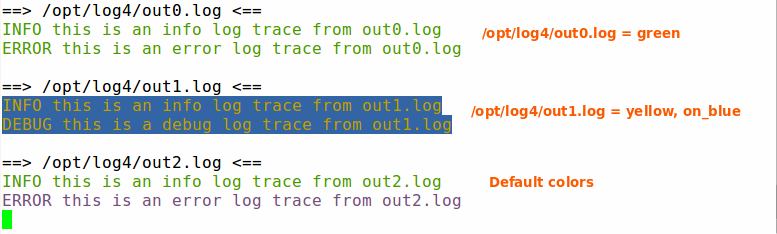
\includegraphics[scale=0.60]{multiple_colors.png}
\caption{\logftailer{} each log with its own color scheme}\label{fig:multiple_colors}
\end{figure}



\subsection{Filter Notification}
\label{sec:filter}
With filter you can filter out information you don't want to be printed out 
in the standard output. It would be a mix of tail and grep. You tail the log 
and grep for the information you are interested in. In order to enable that 
feature you need to execute \logftailer{} with the -f option:

\begin{cmd}
  ./log4tail -f[--filter] tracetofilter pathToLogs
\end{cmd}

\subsection{CornerMark Notification}
\label{sec:cornermark}
CornerMark notification will display a colored box in the bottom right side of
the terminal in case a Fatal, Error, Warning or Target trace has been found during the specified
time. In order to activate this type of notification you need to pass the
option cornermark in the command line as follows:

\begin{cmd}
  ./log4tail --cornermark numberofseconds pathToLogs
\end{cmd}
where numberofseconds can be any number. 

Example of what you would see if that notification is activated can be seen in
 \autoref{fig:cornermark}.

\begin{figure}
\centering
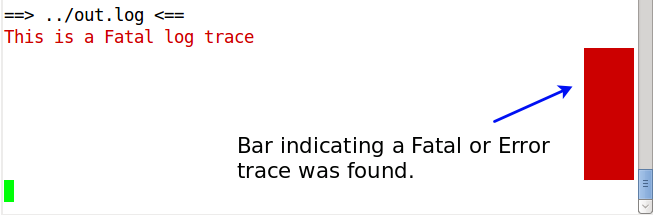
\includegraphics[scale=0.60]{terminalcornermark.png}
\caption{\logftailer{} with cornermark activated}\label{fig:cornermark}
\end{figure}

For Fatals and Errors the mark will be red. For Warnings will be yellow and for Targets 
will be cyan. These three colors are fine for easy identification in either clear terminal
backgrounds or dark ones.

The motivation for having a corner mark is when you need to go for a break and
want some kind of visual alert when something goes wrong. The visual alert will
be displayed for the number of seconds you specify in the command line, so it
is always advisable to be a number greater than the number of seconds you'll be
out of your desktop. 

\subsection{Mail Notification}
\label{sec:mailnotification}
\logftailer{} has an SMTP email client built-in if you want to be notified by email.
Mail notification is used when you want to be notified by email when a target or level (error or fatal) has been found 
in the logs. It is very useful when you are tailing for long hours and you cannot take 
a look at the screen from time to time. It's not necessary to run in silent mode anymore 
to use this action.
This action can be triggered by specifying the command line option -m and
specifying the mail details in a configuration file. 

\begin{cmd}
 ./log4tail -m [--mail] -c [--config] [[-t [--targets] 'regex1,...,regexN'] pathToLogs
\end{cmd}

\textbf{You'll need to provide a configuration file} with the following key parameters:

\begin{verbatim}
 mail_username = yourusername
 mail_hostname = youremailhostname 
 mail_port = port
 mail_ssl = True or False
 mail_from = Email from, it can be the same as your to address 
 mail_to = Email to where you will receive the alerts
\end{verbatim}
The password will be asked during runtime to avoid being left 
in plain ascii in the configuration file. For SSL connection you will need a Python 2.6 runtime, otherwise 
mail\_ssl should be left to False.

If an alert is raised, you will receive an email from mail\_from with the subject ``Log4tailer 
alert'' for easy filtering.

\logftailer{} works with SMTP Google email accounts\footnote{Using SMTP SSL connection. For SMTP SSL
connectivity you'll need a Python 2.6 runtime, as Python 2.4 does not support it.} if you have one. 
In \autoref{fig:mailalert} you can see how it looks like.

\begin{figure}[hb]
%\centering
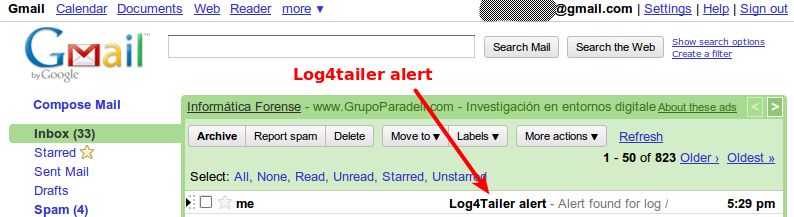
\includegraphics[scale=0.55]{emailalert.png}
\caption{\logftailer{} email alert in gmail}\label{fig:mailalert}
\end{figure}


I have not tested \logftailer{} 
with \textbf{sendmail}. For that you would have to configure sendmail to accept smtp localhost connections. 
Explaining that is out of the scope of this document. You can take a look in the sendmail documentation 
book in the Sendmail Consortium webpage at \href{http://www.sendmail.org}{http://www.sendmail.org}.

\subsubsection{Flood control}
In order to avoid being sent lots of notification emails when a flood of undesirable log traces
turn up, log4tailer has a way to control that by means of a 60 second gap, which means that non desirable 
levels that happen within that gap are not notified. After that expiration time, the first undesirable log 
trace to be found will be notified, triggering again a 60 second gap period. 
 
\subsubsection{When should I use Mail notification}

MailAction would be like having additional eyes taking a look at the logs. That means, that you can take 
a rest from time to time basically. If something is found, then 
you are notified. At this stage, it will notify errors and fatals, considered to be non desired levels in 
an application. Along with that, you can specify a series of patterns (regexes), log4tailer's targets,
that if found could mean that the application is not behaving as expected. In that specific case, you will 
get notified as well.
  
\subsection{Inactivity Notification}
\label{sec:inactivitysection}
Inactivity monitors for inactivity time in the logs. Inactivity as of this release 
will just send an emphasized line in the standard output notifying that there has been 
a lot of inactivity in that log. The inactivity time must be provided in the command line 
with the -i parameter followed by the number of seconds of inactivity to be monitored in the log.
If there has not been any activity for the number of seconds given, \logftailer{} will print 
an emphasized line in the standard output.\\
As an example:\\
\emphlogtrace{{Inactivity in the log for 5.99955296516 seconds}}
 
The command line interface to activate the inactivity monitoring is:
\begin{cmd}
 ./log4tail -i [--inact] numberinseconds pathToLogs
\end{cmd}

\subsubsection{Inactivity Mail Notification}
If you want a notification by email when inactivityAction is raised, just specify in the 
config file:
\begin{verbatim}
 inactivitynotification = mail
\end{verbatim}
By default is notification to the standard output as shown before. 

\subsection{Executor}
\label{sec:executor}

The executor is another type of notification. \logftailer{} will execute a program provided 
by the user if the levels Error, Fatal or Critical have been found in the log trace. The user 
must provide the command line option \emph{--executable} along with a config file specifying 
the key \emph{executor} with value the program you want log4tailer to execute and its parameters 
separated by whitespaces. You can specify a couple of place holders as well, where the first will 
be the log trace found and the second the log path where the trace was found.

\begin{cmd}
 ./log4tail --executable -c configfile pathToLogs
\end{cmd}

where in configfile you could write something like:

\begin{verbatim}
 executor = anyscript %s %s 
\end{verbatim}

Where anyscript can be any program accepting two parameters, namely, lograce and log path. The script 
you provide, of course, will need to have execution permissions for the user 
owning the \logftailer{} process. 

As a simple example, if you cannot configure SMTP for log4tailer, then you could 
setup a script to use the \emph{mail} linux command line to send you an email by means of sendmail.

\subsection{Poster notification}
\label{sec:poster}
The poster notification is basically a REST client built in \logftailer{}. That will open 
the possibility to communicate with a centralized web server with a frontend. Poster 
notification will register to the server and notify all those fatal, critical, errors or 
targets found in the log. 
\begin{cmd}
 log4tail --post -c configfile.txt pathToLogs
\end{cmd}
where in the configfile.txt you will need to specify the following parameters:
\begin{verbatim}
 server_url = url to the server
 server_port = port
 server_service_uri = /where/go/notifications
 server_service_register_uri = /register/log4tailer/toserver
 server_service_unregister_uri = / unregister/log4tailer/fromserver
\end{verbatim}


\section{Pause Modes}

\label{sec:PauseModes}As of release 1.2 \logftailer{} includes pausemodes feature. You will be able 
to pause or freeze the output by a number of seconds if an specific level or target 
has been found. In order to enable pausemodes, you must configure them in a config file 
providing any of the following keys\footnote{the keys are case insensitive, so is the same pauseDEBUG or pausedebug\ldots} :
\begin{verbatim}
 pausedebug = secondsfordebug
 pauseinfo = secondsforinfo
 pausewarn = secondsforwarn
 pauseerror = secondsforerror
 pausefatal = secondsforfatal
 pausetarget = secondsfortarget
\end{verbatim}
You specify only those ones you want to use.
For instance, if we want to freeze the output momentarily (one second) for warnings:
\begin{verbatim}
 pausewarn = 1
\end{verbatim}
Then, we should run log4tailer like:
\begin{cmd}
./log4tail -c yourconfig /pathToLogs
\end{cmd}
Pausetarget keyword will pause the output for any regex found in the log when running log4tailer with -t option.


\section{Reporting}
Every time we finish the tailing, log4tailer will output a report, specifying how long 
log4tailer has been running and the number of events for debug, info and warn. In case of 
error and fatal, it will provide the timestamps when they were found and their corresponding logtrace.
Example:
\begin{verbatim}
Analytics: 
Uptime: 
0.0 years 0.0 days 0.0 hours 0.0 mins 45.9482619762 secs 
Report for Log out.log
Levels Report: 
FATAL:
ERROR:
15 May 2009 17:17:43=>> There was an error here
15 May 2009 17:17:44=>> There was another one in here
15 May 2009 17:17:45=>> Oops, another one
WARN:
4
INFO:
9
DEBUG:
14
TARGET:
3
OTHERS:
18 Jul 2010 11:45:44=>> Inactivity action detected
Ended log4tailer, because colors are fun
\end{verbatim}

\subsection{Reports by email}
If you want a report by email after a given amount of time, then you can do that by means 
of the config file. There are two values that can be setup, namely:
\begin{verbatim}
 analyticsnotification = mail
 analyticsgaptime = 10.5
\end{verbatim}
If these two values are uncommented, then you will be required to provide the mail 
details in the same configuration file, please check the \autoref{sec:mailnotification}. The analyticsgaptime should be given in seconds, by default is 3600 seconds (1 hour). 
You'll receive a report after that period. After that period the statistical information is 
flushed and then sent again once the gap notification time is expired and so on.
In \autoref{fig:emailnotification} %in page \pageref{fig:emailnotification}, 
you can see an email report notification in a Google gmail account.

\begin{figure}
%\centering
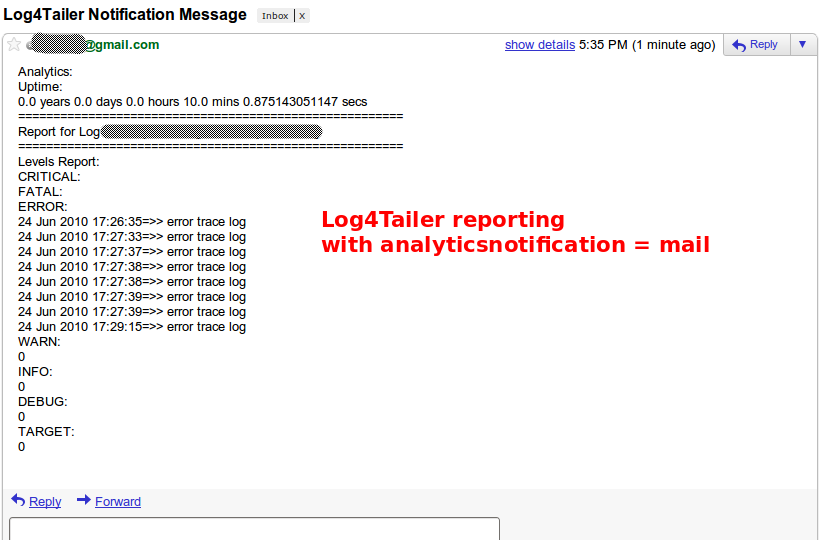
\includegraphics[scale=0.50]{emailnotification.png}
\caption{\logftailer{} email report notification}\label{fig:emailnotification}
\end{figure}


\subsection{Reports to a file}
\logftailer{} can give you a report to a file if you want to. Just provide the
analyticsnotification in the configuration file pointing to the reporting file
(full path). An example of that would be:
\begin{verbatim}
 analyticsnotification = /opt/reportlog4tailer.txt
 analyticsgaptime = 10.5
\end{verbatim}

\section{Silent Mode}
Silent mode, tails the logs in the background (daemonized tailer) and triggers
the Mail notification, notifying if error, fatal or any target has been found in the logs. 
\begin{cmd}
 ./log4tail -s -c [--config] configfile [-t [--targets] 'regex1,..,regexN'] fullPathToLogs
\end{cmd}
\logftailer{} will require a configuration file with your email details. Please take a look 
at the \autoref{sec:mailnotification} where specifies the key parameters 
that need to be specified. It is very important to note that the path to the logs must be the 
full path, no relative. That's because when \logftailer{} enters in daemonized mode, it switches 
to the root directory closing all buffers and detaching itself from the terminal, in other words, 
it becomes a real daemon. As a consequence, it is not necessary to execute it with the nohup 
Linux command line tool.

\subsection{Silent Mode when no access to email notification}
\logftailer{} provides the no-mail-silence optional command line parameter, where it enters in 
daemonized mode with no notification setup. It will be up to the user to setup some type of 
notification by means of a configuration file. Actually, this option is thought to be used along 
with the -config parameter where you can specify some notification. One of the scenarios would be 
when you want automatic monitoring when the server you are running \logftailer{} has no ports available 
for email notification. You could provide a config file with \emph{analyticsnotification} pointing to 
a file where \logftailer{} would do a report of the logs status every \emph{analyticsgaptime} seconds 
or one hour by default.

\begin{cmd}
 ./log4tail --no-mail-silence -c [--config] configfile fullPathToLogs
\end{cmd}


\section{Coloring Standard Input}
Log4tailer can colorize its standard input to the standard output. Main use would be when your application 
does some output and finishes. In order to do that just type:
\begin{cmd}
 yourapplication | log4tail -
 cat somelog.log | log4tail -
\end{cmd}
You can use the \emph{more} Linux/Unix application in order to page the output. Example:
\begin{cmd}
 cat somelog.log | log4tail - | more
\end{cmd}

\section{Tailing last N lines}
You can tail last \emph{N} lines from the log with the \emph{-n} option. Just type:
\begin{cmd}
 ./log4tail -n numberOfLines pathToLog
\end{cmd}
and it will output the last \emph{numberOfLines} from the log colorizing the corresponding levels.

\section{SSH Tailing}
SSH Tailing or remote tailing will allow you to tail multiple remote logs from different hosts. As of now, only 
PrintAction is available, so you'll be able to tail multiple remote logs in a colorful way as specified in 
section \ref{sec:PrintAction}. In order to tail remotely you'll need to pass as a parameter the -r option 
along with some config file parameters:
\begin{cmd}
 ./log4tail -r -t targets -c yourconfig.txt
\end{cmd}
In your configfile you must provide the following parameters:
\begin{verbatim}
 sshhostnames = hostname0, hostname1, hostnameN-1
 hostname0 = username0, /var/log/log0, /var/log/log1, /var/log/logN-1
 hostname1 = username1, /var/log/log0, /var/log/log1, /var/log/logN-1
 hostnameN-1 = usernameN-1, /var/log/log0, /var/log/log1, /var/log/logN-1
\end{verbatim}
Where:
\begin{itemize}
\item \textbf{sshhostnames} is a comma separated values of hostnames
\item every \textbf{hostname} must be a parameter itself where first value should be its username and 
then the logs you want to tail.
\end{itemize}
By default log4tailer will try to authenticate by using your rsa key under your
$\sim$/.ssh/id\_rsa key if it exists, otherwise it will use normal username, password
authentication. If you want to use another rsa key other than the default
id\_rsa key then you can provide one in the config file by using the rsa\_key
parameter. Example:
\begin{verbatim}
 rsa_key = /home/youruser/.ssh/myrsakey
\end{verbatim} 
rsa\_key value must be the full path to the rsa\_key.

Some considerations are to be taking into account. As of now, remote tailing \textbf{only} provides 
PrintAction along with targets, that means that you will be able to tail with colors and emphasize those log traces 
that match the comma separated regexes provided with -t. Besides, you'll be able to use 
pauseModes set up in the config file as explained in section \ref{sec:PauseModes}.

To finish, just Ctrl-c and it will close all channels opened to communicate to the remote hosts. 

\subsection{Dependencies for SSH tailing}
It is very important to note that for remote tailing, you'll need to install the \textbf{paramiko module}, 
available in major Linux distributions. In most of them is available under the name of python-paramiko. In 
Debian systems, you'll need to type:
\begin{cmd}
 sudo apt-get install python-paramiko
\end{cmd}

\section{Configuration file}
Config file is provided fully documented for convenience; just uncomment those lines you are interested 
to enable and modify them for your specific purposes. In order to enable those values in the config file, 
you must notify that to \logftailer{} as a parameter in startup time.
\begin{cmd}
 ./log4tail -c yourconfig.txt logs
\end{cmd}
If you always use the same configuration file, you can copy it in your HOME directory as \emph{.log4tailer} and log4tail will read it next time you execute the program, even if you 
don't provide the -c option.

The config file provided for convenience is called log4tailerconfig.txt and is quoted below:
\begin{verbatim}

# Optional config for log4tailer
# to activate it
# log4tail -c config yourlogs

# ====================================================
# Custom colours for every level. Available 
# colours are: red, green, yellow, blue, magenta, cyan 
# and white. Uncomment to override the default ones.
# ====================================================

# warn = yellow, on_cyan
# error = magenta 
# fatal = red, on_green
# info = green
# debug = black

# ================================
# targets: which lines do you want 
# to emphasize by using regexes
# uncomment and provide your values.
# ================================

# targets path/to/log0 = regex0,regex1,regex2 | coloregex0, coloregex1, ...
# targets path/to/log1 = regex0,regex1,regex2 | coloregex0, coloregex1, ...

# ======================================================
# Every log with its own color scheme, overriding colors 
# for every level.
# ======================================================

# /path/to/log0 = yellow
# /path/to/log1 = red

# ======================================================
# Pause the output by the number of seconds specified if 
# a level or target has been found. Uncomment the ones 
# you want. The value can be any number in seconds. 
# ======================================================

# pausedebug = 4
# pauseinfo = 2
# pausewarn = 1
# pauseerror = 1
# pausefatal = 1
# pausetarget = 1


# ======================================================
# Mail details 
# ======================================================

# mail_username = yourhostusername
# mail_hostname = mailhostname
# mail_port = 25
# mail_ssl = True or False
# mail_from = any from address
# mail_to = alerts will be sent in the address you specify in here


# ===================================================================
# Inactivity notification, by email or stdout.
# Possible values can be "mail" or "print". By default is "print".
# ===================================================================

# inactivitynotification = mail

# ====================================================================
# Analytics notification. You can make log4tailer send you 
# a report every analyticsgaptime seconds. By default it will be 
# printed out once finished. Uncomment analyticsnotification to 
# report by email or to a file. Another possible value can be "print".
# ====================================================================

# analyticsnotification = mail
# analyticsnotification = fullPathToaFile
# analyticsgaptime = 10.5


# ==============================
# SSH Tailing parameters
# ==============================

# sshhostnames = hostname0, hostname1, hostnameN-1
# hostname0 = username0, /var/log/log0, /var/log/log1, /var/log/logN-1
# hostname1 = username1, /var/log/log0, /var/log/log1, /var/log/logN-1
# hostnameN-1 = usernameN-1, /var/log/log0, /var/log/log1, /var/log/logN-1

# rsa_key defaults to ~/.ssh/id_rsa, if that's not your case then 
# provide yours

# rsa_key = fullpathToRsaKeyName 

\end{verbatim}

\newpage
